\section{Grundaufbau}
    Der Ballwerfer ist so konzipiert, das er aus einem fix stehenden Basismodul besteht, 
    welches in der Mitte des Startbereiches positioniert wird. Die Abwurfeinheit, welche 
    den Ballwurfmechanismus und die Ballzuführung beinhaltet, ist auf dem Basismodul 
    drehend gelagert. Weiter ist auch das Smartphone für die Korberkennung und alle 
    Steuereinheiten auf dem Basismodul angebracht. Das Startsignal wird mittels WLAN 
    von einem externen Notebook übertragen.\\
    \\
    Der ganze Aufbau des Ballwurfmechanismus ist sehr simple gehalten. Er besteht 
    hauptsächlich aus zwei $5\si{\milli\meter}$ dicken Acrylglasplatten, in welcher alle mechanischen 
    Vorrichtungen gelagert sind. Durch diesen Aufbau können Änderungen schnell und 
    einfach angepasst werden. Die Ausrichtung des Abwurfmechanismus erfolgt durch 
    einen sehr flachen Steppermotor, welcher in der drehenden Abwurfeinheit angebracht 
    ist. Dadurch wird die Bauhöhe des Ballwerfers tief gehalten, was einen grossen 
    Stabilitätsvorteil bietet. Die Drehachse der Abwurfeinheit ist an der Spitze des 
    Ballwerfers mit einem Bolzen angebracht. Somit bleibt die Abwurfposition der 
    Tennisbälle konstant am gleichen Ort. Die Tennisbälle werden durch zwei 
    Beschleunigungsräder beschleunigt. Die Beschleunigungsräder werden je einzeln 
    über eine Übersetzung mit einem Brushlessmotor auf Touren gebracht. Die Beschleunigungsräder 
    drehen gegenläufig und die Tennisbälle werden dazwischen hindurchgeführt und 
    abgeworfen. Die Zuführung der Tennisbälle zu den Beschleunigungsräder erfolgt mit 
    einem Förderband. Das Förderband transportiert die Bälle mit einer 
    konstanter Geschwindigkeit zu den Beschleunigungsräder, damit alle Tennisbälle die 
    gleiche Startenergie aufweisen. Dadurch ist eine gleichmässige Wurfweite und eine 
    hohe Reproduzierbarkeit gewährleistet.
    
    
    \subsection{Herstellung Acrylglas}
		Für die Seitenwände, die Zahnscheibe und für die Verbindungsstege wurde eine 
		$5\si{\milli\meter}$ Dicke Acrylglas (PMMA) Platte verwendet. Die Konturen 
		wurden mit dem Laser an der HSLU gefertigt. Damit der Laser die Daten lesen 
		konnte, wurde aus dem CAD eine dxf-Datei erstellt. Um die Nachbearbeitung 
		möglichst gering zu halten, wurden auch die Lager- und Durchgangsbohrungen 
		für die Schrauben direkt auf das Fertigmass gelasert. Die Lager passten dabei 
		sehr genau in die Bohrungen, sodass sie ein wenig klemmten und trotzdem keine 
		starken Spannungen erzeugten, die allenfalls zu Rissen führen könnten. Dies 
		wurde im Vorfeld getestet (siehe Doku PREN 1). Die einzigen Nachbearbeitungen 
		waren die seitlichen Bohrungen an den Seitenwänden und an den Spannelementen. 
		Dabei musste auf eine gute Kühlung geachtet werden, da die Restwandstärke nur 
		noch je $1\si{\milli\meter}$ beträgt und das Acrylglas sehr schnell weich wird. 
		Ebenfalls musste die Schnittgeschwindigkeit für das Bohren drastisch gesenkt 
		werden gegenüber einem normalen Kunststoff wie PE. Die seitlichen Bohrungen an 
		den Seitenwänden wurden auf einer Universalfräsmaschine gefertigt, die über eine 
		horizontale Frässpindel verfügt (siehe Abbildungen \ref{fig:Acrylglas_1} und 
		\ref{fig:Acrylglas_2}). Die Bohrungen für die 
		Elekronikprints und andere kleine Anpassungen wurden ebenfalls erst nach dem 
		Lasern gefertigt. Zum Beispiel die Ansenkungen für die Schraubenköpfe oder bei 
		den Elekronikprints weil der endgültige Platz noch nicht festgelegt war.
		\begin{figure}[h!]
			\begin{minipage}[hbt]{0.5\textwidth}
		   		\centering
		   		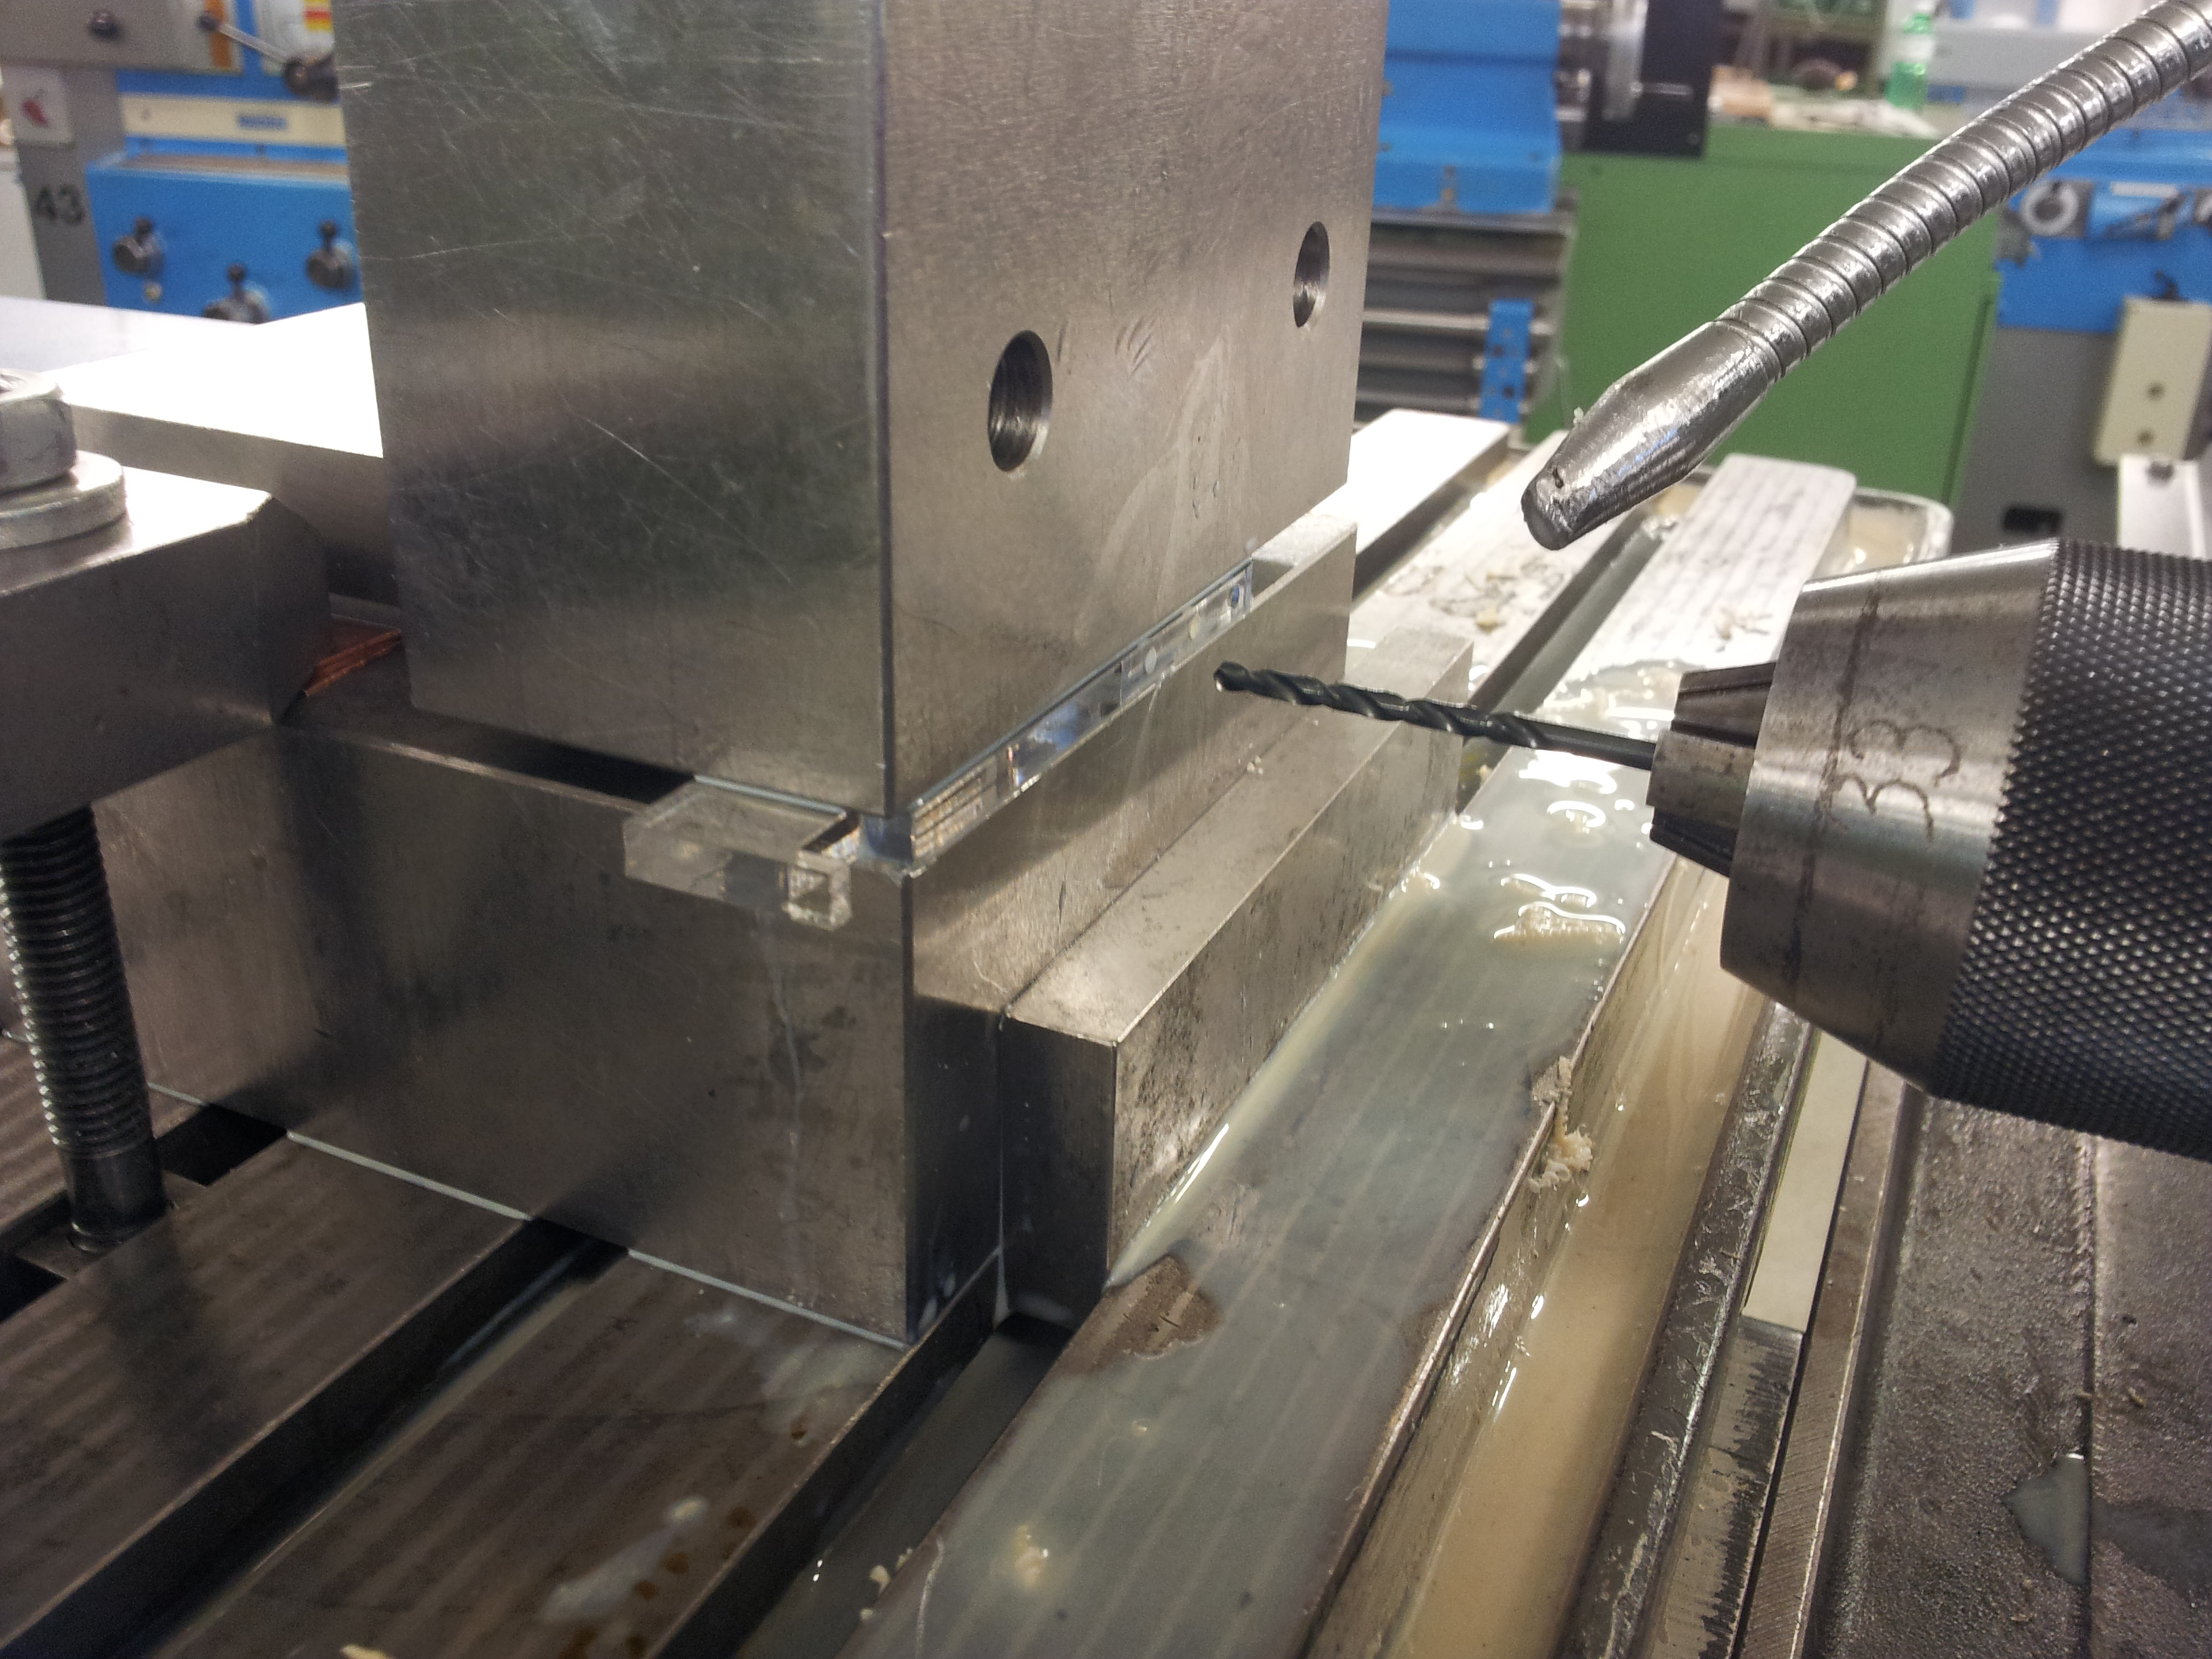
\includegraphics[width=1\textwidth,clip,trim= 0mm 0mm 0mm 0mm]
		   		{Enddokumentation/Bilder/Herstellung_Acrylglas_1.jpg} 
		   		\caption{Herstellung der Acrylglas-Teile}
		   		\label{fig:Acrylglas_1}
			\end{minipage}
			\hfill
			\begin{minipage}[hbt]{0.5\textwidth}
		   		\centering
		   		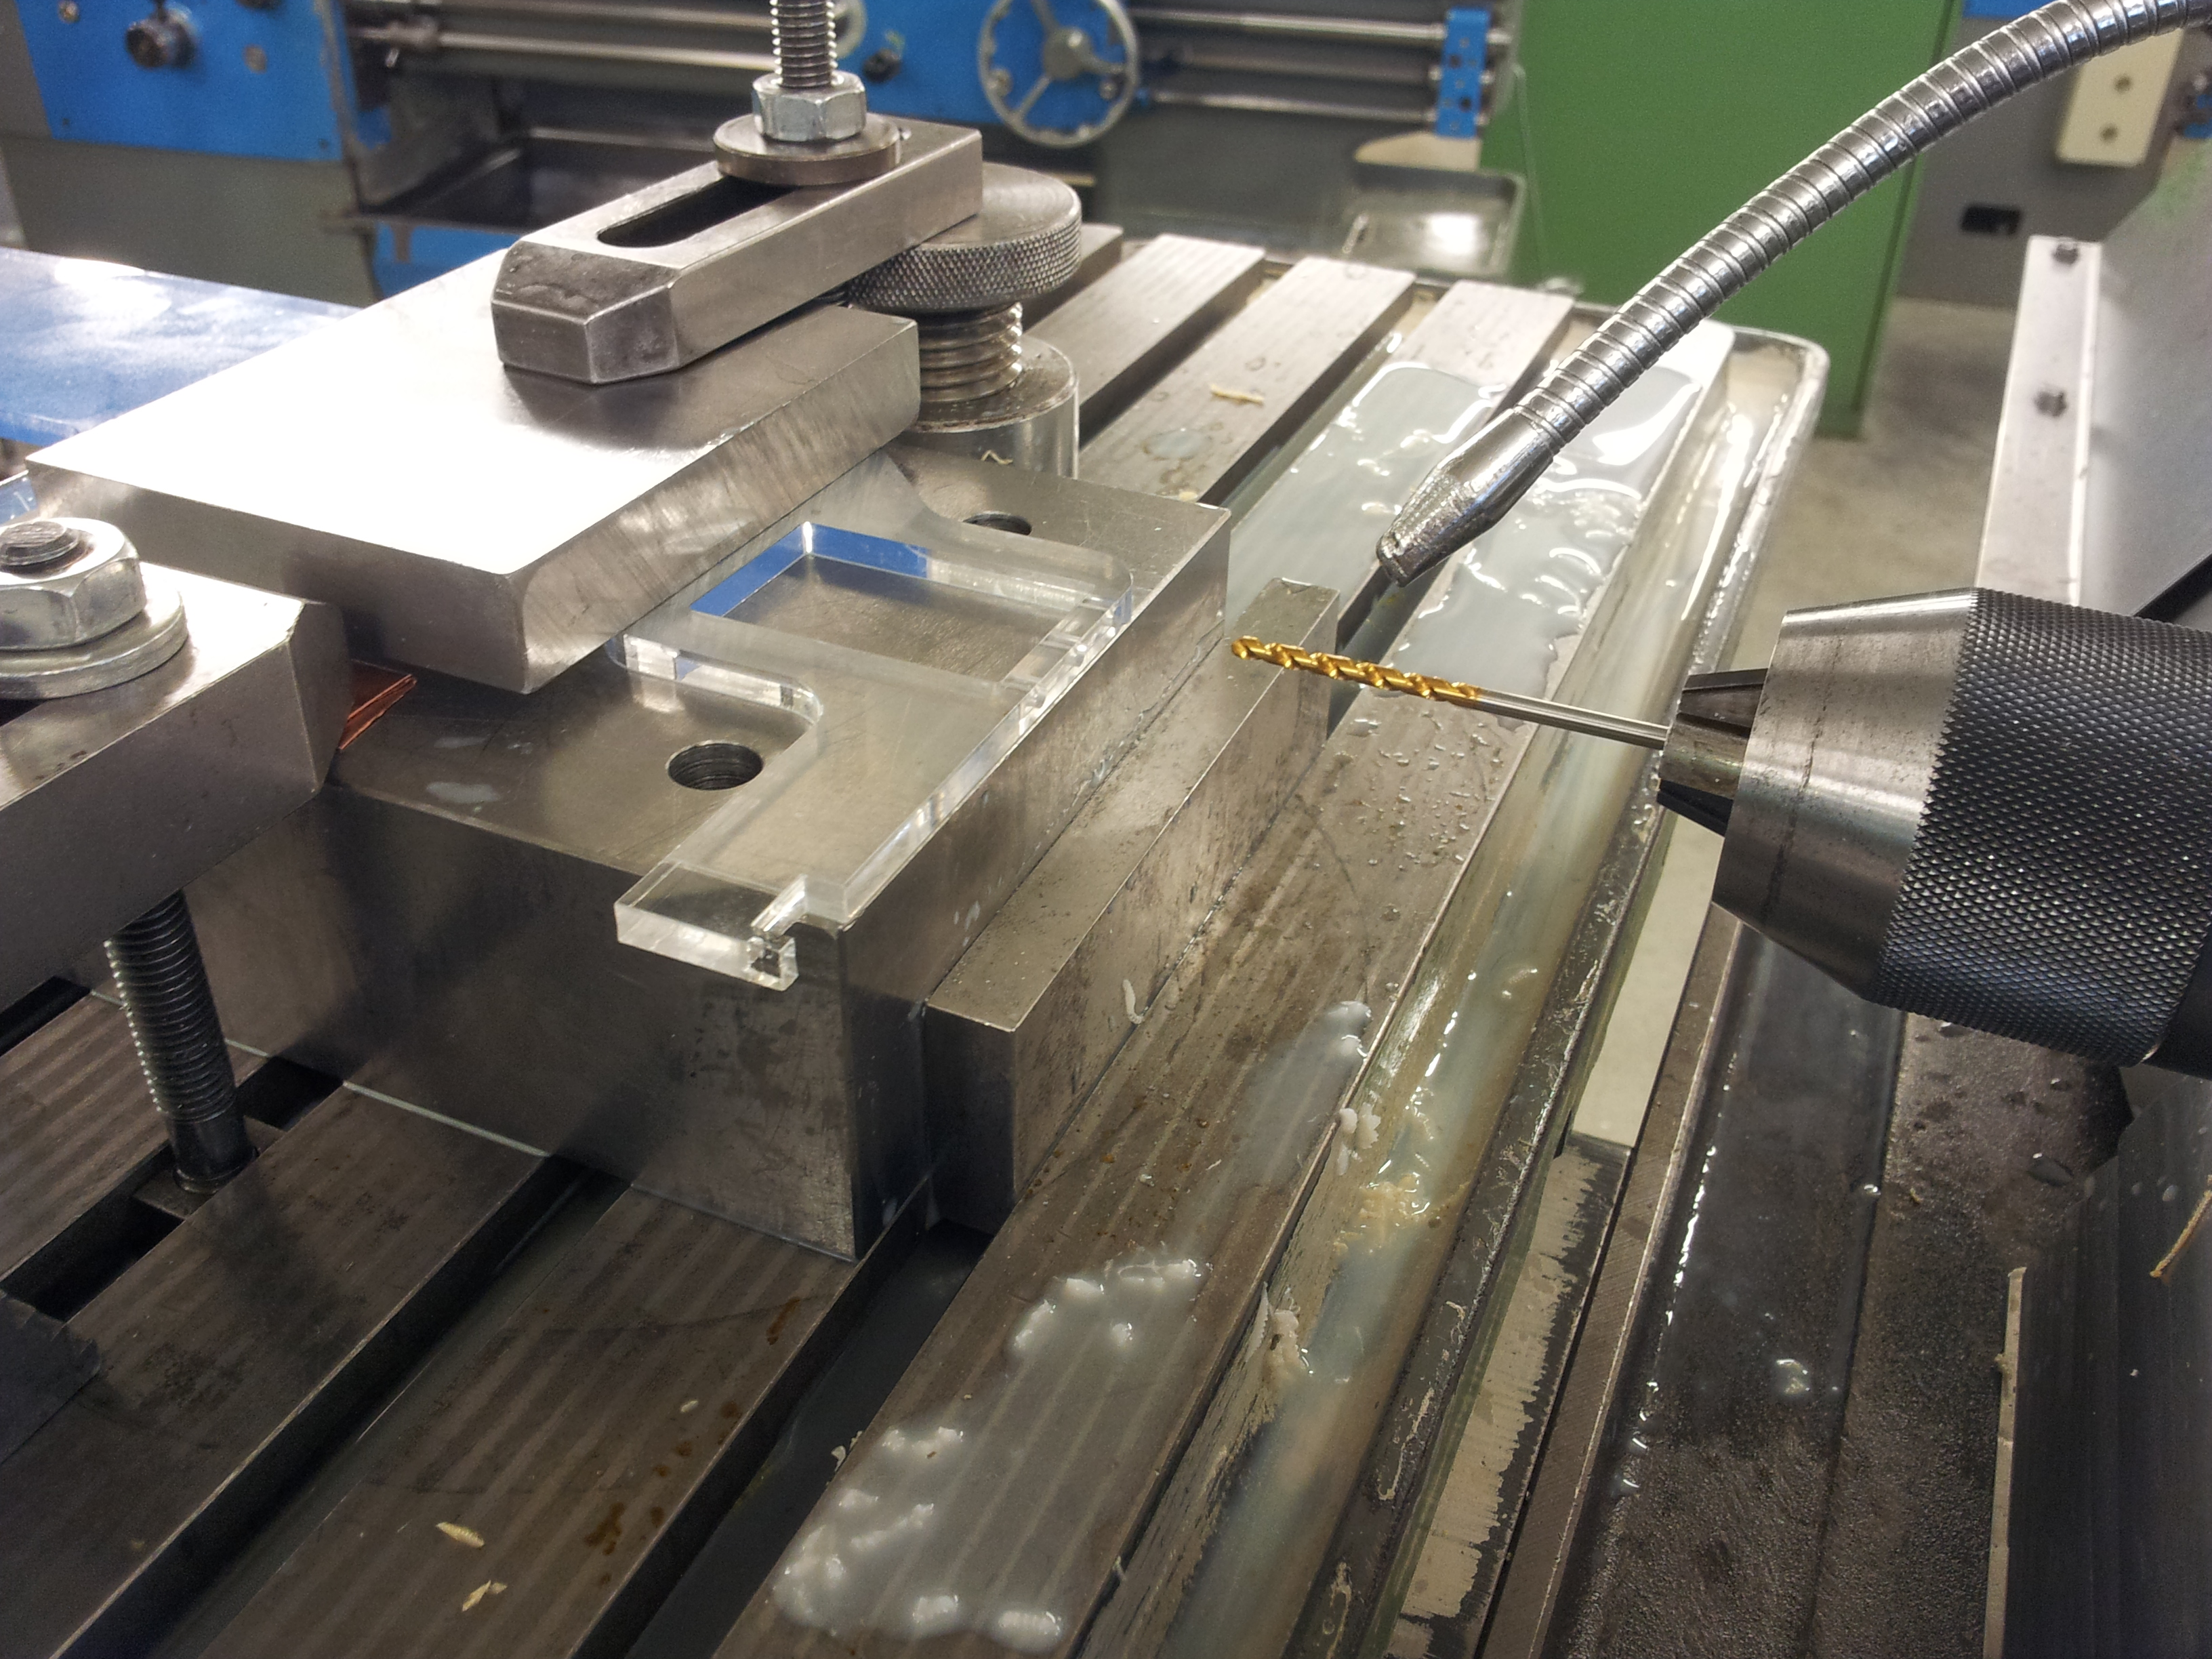
\includegraphics[width=1\textwidth,clip,trim= 0mm 0mm 0mm 0mm]
		   		{Enddokumentation/Bilder/Herstellung_Acrylglas_2.jpg} 
		   		\caption{Herstellung der Acrylglas-Teile}
		   		\label{fig:Acrylglas_2}
			\end{minipage}
		\end{figure}
		
		
    \subsection{Hauptcontroller}
        Die gesamte Hardware wird über das Freedom-Board\footnote{Development-Board vom 
        Hersteller Freescale, Typ FRDM-KL25Z} gesteuert. Dieses Board hat einen internen UART\footnote{\textbf{U}niversal \textbf{A}synchronous \textbf{R}eceiver 
        \textbf{T}ransmitter, eine serielle Schnittstelle} to USB Converter, über diesen 
        das Smarphone mit dem Freedom-Board kommuniziert. Die Software des Boards besteht aus einem 
        Betriebssystem, dessen Haupttask kontinuierlich den UART Eingangspuffer abruft 
        und die angekommenen Befehle ausführt. Ein wichtiger, nur einmal gebrauchter Task, 
        ist die Initialisierung des Stepperboards, siehe Anhang Kapitel \ref{sec:StepperAnsteuerung}. Der Controller 
        verfügt über zwei SPI\footnote{Serial Peripheral Interface, ein synchroner serieller Datenbus }-Schnittstellen. An einer ist das besagte Stepperboard und 
        an der anderen die beiden Brushless-Boards angeschlossen. Weiter wird ein PWM\footnote{pulse width modulation}-Port 
        verwendet, um den Motor der Ballnachführung anzutreiben, siehe Kapitel 
        \ref{sec:Foerderband}.  

   
    \subsection{Spannungsversorgung}       
        \begin{wrapfigure}{r}{0.35\textwidth}
           	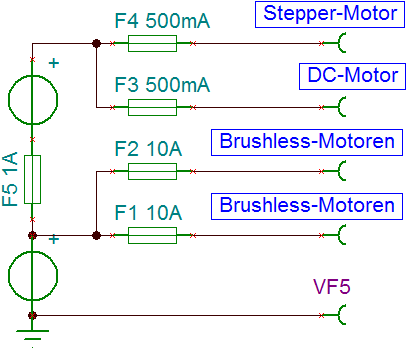
\includegraphics[width=0.35\textwidth,clip,trim=0mm 0.5mm 0mm 0mm]
           	{Enddokumentation/Bilder/BeschaltungNetzteile.png}
           	\centering
           	\caption{Schema der Spannungsversorgung} 
           	\label{abb:Spannungsversorgung}
        \end{wrapfigure}
        Gemäss Datenblatt sind die verwendeten Brushless-Motoren mit einer Versorgungsspannung 
        von $12\si{\volt}$ bei einem maximalen Strom von $11\si{\ampere}$ spezifiziert. 
        Der Steppermotor und der DC-Motor sind gemäss Datenblatt für eine Betriebsspannung 
        von $24\si{\volt}$ ausgelegt. Die Spannungsversorgung wird mit zwei Server-Netzteile 
        realisiert, die je $12\si{\volt}$ mit maximal $60\si{\ampere}$ liefern. Aus 
        Sicherheitsgründen wird für jeden Motor eine separate Sicherung verwendet. Das Schema 
        in Abbildung \ref{abb:Spannungsversorgung} zeigt, wie die Spannungsversorgung 
        realisiert ist. Das Freedom-Board wird über USB vom Akkumulator des Smartphone 
        gespeist. Sämtliche Datenblätter zu den verwendeten Motoren sind im Anhangsdokument 
        angefügt. Das zweite Netzteil wurde so umgebaut, dass es potentialfrei arbeitet. So 
        ist es möglich, dass es die $12\si{\volt}$ auf die Spannung des ersten Netzteils 
        generieren kann. Die Sicherung zwischen den beiden Netzteilen ist als Sicherheit 
        hinzugefügt für den Fall, dass es Probleme mit der Potentialfreiheit gibt.	